\vspace{0.5cm}
Un conteneur est un ensemble de processus isolés du reste du système tout en étant léger.Docker est une technologie de conteneur basé sur la virtualisation de Linux LXC (Linux Containers)
\vspace{0.5cm}
Le Docker est un outil utilisé pour :
\begin{itemize}
	\item Répondre à des besoins de production
	\item Unifier les environnements des différents développeurs et les rendre fonctionnels
	\item transporter de manière fluide les applications de l’environnement de développement jusqu’à l’infrastructure de production.
\end{itemize}
Il partage les ressources avec le système hôte,démarre plus rapidement que les machines virtuelles,améliore le cycle de déploiement.En terme de déploiement continu ,il limite les mises à jour au container qui nécessite de l'être.
\section*{Les composants de Docker}
\begin{itemize}
	\item \textbf{Docker registry} :C'est une bibliothèque d'images d'applications.Il met à disposition les images ,s'occupe de leur  versionning,permet de très facilement récupérer un conteneur en HTTP.On peut partager des images à d'autres personnes grâce aux registry.
	\item \textbf{Docker Demon Client}: Il crée les environnements LXC sur le serveur, et s’occupe de paramétrer et d’instancier le conteneur.
	\item \textbf{Dockerfile}
	C'est un script qui contient une liste d'instructions pour construire chaque etape ou couche de l’image.Dans ce fichier on définit l’image qu’on veut utiliser comme base.C’est l’équivalent d’un package json ou node.js en PHP.Voici les étapes de construction d'une image:
	\begin{itemize}
		\item
		\item\textbf{FROM} nom de l'image de base
		\item\textbf{RUN} apt-get update (par exemple)
		\item\textbf{ADD} /chemindufichier
		\item\textbf{WORKDIR} repertoire 
		\item\textbf{EXPOSE } port
		\item\textbf{VOLUME} dossier à partager
	\end{itemize}
	\vspace{0.5cm}
	Et enfin pour transformer le fichier en une image docker on utilise la  \textbf{\textit{docker build -t}} nom de l'image.
	\vspace{0.5cm}
	\textbf{WORKDIR} : équivalent à la commande cd en ligne de commande ,elle permet de modifier un répertoire
\end{itemize}
Introduction
Dans le but de mettre à niveau les compétences des stagiaires il nous a été demandé de nous lancer la recherche et l'exercie d'une technologie utilisée dans les entreprises qui respectent le système du devOps.Ainsi notre travail a été basé sur Docker.De nos jours,la technologie des conteneurs reste la plus déployée pour la mise en place des outils dédiés au Devops. les Dockers rendent  la tache facile aux développeurs car ils permettent aux applications d'etre indépendantes des infrastructures.Mais avant d'aller dans le sujet 
Parlons d’abord virtualisation.
La virtualisation est un processus qui permet de créer d'autres machines virtuelles ayant les caractéristiques d'une machine physique et qui emploient les ressources informatiques de cette dernière(mémoire RAM,CPU etc...).Il s’agit de créer un système hôte pour qu’il ait les mêmes propriétés que ce dernier
%\vspace{0.5cm}
Une \textbf{machine virtuelle} : c’est une solution qui vient rajouter de la puissance aux pc ,aux hôtes pour effectuer les taches lorsque celles ci demandent assez de ressources.Elle permet donc d'exécuter plusieurs applications sur la même machine par exemple.
%\vspace{0.5cm}
Un \textbf{hyperviseur}:c'est une couche logicielle qui permet de gérer l'allocation des ressources.
Mais il arrive que souvent les applications qui sont installées  ne consomment pas toutes les ressources disponibles sur les machines virtuelles.Ce qui fait donc du gaspillage.Cependant, les hyperviseurs de machines virtuelles reposent sur une émulation du hardware, et requièrent donc beaucoup de puissance de calcul. Pour remédier à ce problème, de nombreuses firmes se tournent vers les containers, et par extension vers Docker.Avec Docker , les applications peuvent s'exécuter au sein du système d'exploitation mais de manière virtuelle et isolée,ce qui n'est pas le cas des machines virtuelles.
%Alors que la virtualisation consiste à exécuter de nombreux systèmes d’exploitation sur un seul et même système, les containers se partagent le même noyau de système d’exploitation et isolent les processus de l’application du reste du système.
%  les hyperviseurs doivent créer une copie complète du système d’exploitation qui fonctionne sur un espace matériel virtuel.sur un espace matériel virtuel. L’hyperviseur est donc responsable de tous les échanges de données. Exécuter plusieurs machines virtuelles sur un même serveur demande de grosses performances et un nombre suffisant de ressources pour assumer plusieurs machines virtuelles.
\section*{Les catégories de conteneurs} 
Il existe plusieurs technologies de conteneurs adaptables pour les différents systèmes d'exploitation.Ainsi nous avons :
\begin{itemize}
	\item Docker Desktop uniquement pour Mac ou Windows
	\item Docker Community Edition: est idéal pour les développeurs et les petites équipes qui souhaitent se familiariser avec Docker et expérimenter des applications basées sur des conteneurs.
	\item  Docker Enterprise Edition
\end{itemize}
\subsection*{Installation}
\begin{itemize}
	\item Sur Linux: aller sur le site \textbf{https://docs.docker.com/install/linux/docker-ce/ubuntu/}.
	\vspace{0.5cm}
	A la fin on obtient:
	\begin{figure}[!h]
		\centering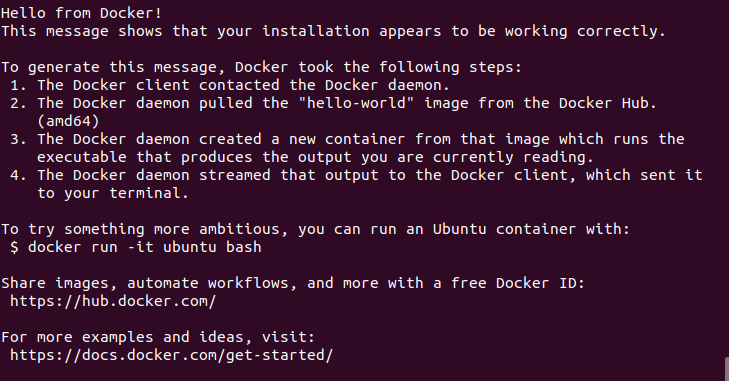
\includegraphics[scale=0.5]{images/cap.png}
	\end{figure}

	\item Mac ou Windows: Aller sur le  http://hub.docker.com  et créez votre compte puis suivez les instructions.
\end{itemize}
\section*{Stockage d'image}
Une image Docker est un empilement de couches appelées \textbf{layers}.Pour stocker une image on part d’une image de base d’un OS et ensuite on installe des composants (en couches) Mysql, Apache ainsi de suite.Cela rend avantageux dès lors qu’on peut remplacer les versions des couches.Nous avons des outils spécialisés dans le stockage d'image précisement le Docker Hub ,qui est un service de Docker Inc.Voici quelques commandes usuelles qui sont utilisées.
\begin{itemize}
	\item\textbf{docker pull }:récupérer une image 
	\item\textbf{docker build }: construire une nouvelle image
	\item\textbf{docker run }: instancier un nouveau conteneur
\end{itemize}
\section*{\textit{Dockers et Devops}}
\vspace{0.5cm}
Imaginez un développeur qui envoie son code à un testeur.Le code ne fonctionne pas sur l'autre système en raison de la différence des environnements.Voilà ce à quoi répond Docker.
\vspace{0.5cm}
Docker s'adapte parfaitement à l'écosystème DevOps, fournissant aux professionnels de DevOps des outils pour accélérer et rationaliser le cycle de vie du développement logiciel.Les Dockers sont facilement transportables sur les serveurs Linux.
\section*{Docker Compose}
Le composant Docker Compose permet de définir la composition des composants au sein d’un container dédié.La différence entre Docker et Docker Compose est que ce dernier peut gérer plusieurs conteneurs.Il permet de les lancer grace à un fichier de configuration écrit en YAML.Ces conteneurs sont décrits comme un ensemble de services.
Voici quelques commandes utiles :
\begin{itemize}
	\item \textbf{docker ps }:affiche toutes les instances de docker qui tournent actuellement sur votre environnement
	\item \textbf{docker-compose ps}:affiche tous les containers qui ont été lancés par docker-compose
	\item \textbf{docker-compose logs (<ID>/<NAME>)}: permet de voir les logs d’un conteneur uniquement, au lieu de voir tous les logs.
	\item \textbf{docker exec -it <NAME>/<ID> <“sh”>/<”/bin/bash”>}: permet de lancer un shell sur votre container.
\end{itemize}

% Le Docker Hub est un outil SaaS permettant aux utilisateurs de publier et de partager des applications basées container via une bibliothèque commune.
Conclusion
Les containers Docker sont à nos jours d'une grande utilité pour les Devops tant à l'ochestration des ressources , qu'à la haute performance d'execution des taches qu'ils fournissent.Ils deviennent donc inlassables dans les processus de déploiement et à l'automatisation. 
